%%%%%%%%%%%%%%%%%%%%%%%%%%%%%%%%%%%%%%%%%%%%%%%%%%%%%%%%%%%%%%%%%%%%%%%%%%%%%%%%
%2345678901234567890123456789012345678901234567890123456789012345678901234567890
%        1         2         3         4         5         6         7         8

\documentclass[letterpaper, 10 pt, conference]{ieeeconf}  % Comment this line out if you need a4paper

%\documentclass[a4paper, 10pt, conference]{ieeeconf}      % Use this line for a4 paper

\IEEEoverridecommandlockouts{}
% This command is only needed if
% you want to use the \thanks command

\overrideIEEEmargins{}
% Needed to meet printer requirements.

% See the \addtolength command later in the file to balance the column lengths
% on the last page of the document

% The following packages can be found on http:\\www.ctan.org
\usepackage{graphics} % for pdf, bitmapped graphics files
\usepackage{epsfig} % for postscript graphics files
%\usepackage{mathptmx} % assumes new font selection scheme installed
%\usepackage{times} % assumes new font selection scheme installed
%\usepackage{amsmath} % assumes amsmath package installed
%\usepackage{amssymb}  % assumes amsmath package installed
\usepackage{ulem}
\usepackage{cite}

\renewcommand{\citedash}{--}

\newcommand{\lorem}{
% .
%   Lorem ipsum dolor sit amet, consectetur adipiscing elit.
%   Nam vitae faucibus risus.
%   Curabitur congue neque ipsum, ac egestas quam porttitor sit amet.
%   Fusce id tempus diam.
%   Donec nibh velit, bibendum eget magna sit amet, tincidunt gravida neque.
%   Praesent dolor felis, sodales quis lorem volutpat, varius varius felis.
%   Maecenas quis ex lobortis, suscipit diam eu, bibendum eros.
%   Integer iaculis ante quis erat facilisis, ac egestas orci condimentum.
%   Sed id metus nibh.
%   Maecenas eget pellentesque enim.
%   Nunc finibus augue quis risus laoreet malesuada.
%   Curabitur suscipit elementum libero, quis feugiat felis suscipit et.
%   Sed vehicula pellentesque sem sed accumsan.
%   Integer congue arcu quis arcu sodales, tempus posuere tortor posuere.
%   Integer libero velit, tristique sit amet dui vel, sollicitudin tincidunt tellus.
}

\title{\LARGE \bf
Indoor Robot Localization with WiFi Signal and Convolutional Neural Networks and Recursive Bayesian Estimation
}


\author{Murat Ambarkutuk$^{1}$ and Tomonari Furukawa$^{2}$% <-this % stops a space
\thanks{$^{1}$Murat Ambarkutuk and $^{2}$Tomonari Furukawa are with Computational Multiphysics Lab, Department of Mechanical Engineering,
        Virginia Polytechnic Institute and State University, US
        {\tt\small $^{1}$murata@vt.edu}, {\tt\small $^{2}$tomonari@vt.edu}}%
}
\begin{document}



\maketitle
\thispagestyle{empty}
\pagestyle{empty}


%%%%%%%%%%%%%%%%%%%%%%%%%%%%%%%%%%%%%%%%%%%%%%%%%%%%%%%%%%%%%%%%%%%%%%%%%%%%%%%%
\begin{abstract}

  This paper presents a robot localization system with WiFi signal where a Deep Learning framework utilized to fully exploit the information from signal maps of various Access Points (AP) available in an environment.
  Similar to conventional systems relying on the fingerprinting technique, the system is consisted of two stages: data acquisition and learning (offline), and localization (online).
  In offline stage, the signal maps for various AP's are constructed via Received Signal Strength (RSS) information and learned by a Convolutional Neural Network, whereas the online stage contains the proposed localization method based on an information fusion technique.
  \textit{Add some result once get it}
\end{abstract}


%%%%%%%%%%%%%%%%%%%%%%%%%%%%%%%%%%%%%%%%%%%%%%%%%%%%%%%%%%%%%%%%%%%%%%%%%%%%%%%%
\section{INTRODUCTION}

  Since WiFi has become ubiquitious, it started being utilized in different applications varying from customer tracking indoors to robot localization. % more varying examples would be good.
  However it is available, the information can be extracted from is prone to (suffers from) being sparse and severely effected by infrasracture of environments where WiFi based systems are deployed.
  Amongst all the applications that WiFi signal can be used, localization is a problem where it is required to have higher level of success in localization accuracy and shorter localization time.
  \textit{The main contributions of this paper is that the proposed technique can handle sparse, noisy RSS measurements acquired from the off-the-shelf AP's under LoS and NLoS situations, while achieving comparable localization accuracy to thes state-of-the-art methods.}

  The success of the systems relying on the WiFi signal, in general, suffers from the phenomenon called Multipath Effect where the AP is not in the direct line of sight and the EM waves from the AP where the received signal is propagated through non-line-of-sight, i.e.~concrete and glass walls.
  Although there is some effort to either model or estimate the Multipath Effect to componsate its effects on the systems~\cite{cai2015identification}, it is still an open problem in the field in order to achieve the same level of success.
  %One way to componsate the multipath effect is to find out the first the time epoch the signal is acquired; however, some of these operations require significant change in hardware so that  \# \#.
  \textit{The proposed system can inherently handle multipath effect, since machine not only can reduce complexity of overall design of the system but also can capture deeper information from the radio maps.}
  % \textit{More explanation regarding the multipath effect is needed here to emphasize that machine learning algorithms can inherently handle it.}

  Another problem with the WiFi signal which makes it difficult to employ it as the main information source is that the signal acquired is not reliable.
  Figure~\ref{fig-sample} shows the acquired RSS information acquired with stationary client from the AP's both line-of-sight and non-line-of-sight positions in time.
  The figure clearly depicts that even for stationary clients, WiFi information \#\textit{gotta mention that deviation makes it not reliable}.
  To be able to extract relatively reliable information, some hardware and software changes proposed to incorporate Channel State Information (CSI) provided by Orthogonal Frequency-Division Multiplexing (OFDM) forming WiFi protocol.
  As~\cite{gao2015channel} suggests/proves, the CSI information provides significantly reliable information.
  However, to be able to acquire CSI information, a specific type of NIC should be used with a specific type of firmware.
  This makes it hard to deploy proposed system on Embedded-devices, IoT's and robotic systems.\textit{, while the proposed system can be deployed to almost-any arbitrary system thanks to the simplicity of the design.}

  % \textit{Nail the idea Machine Learning stuff can be deployed practically everywhere}
  \begin{figure}[thpb]
     \centering
    %  \framebox{\parbox{3in}{We suggest that you use a text box to insert a graphic (which is ideally a 300 dpi TIFF or EPS file, with all fonts embedded) because, in an document, this method is somewhat more stable than directly inserting a picture.
    %  }}
     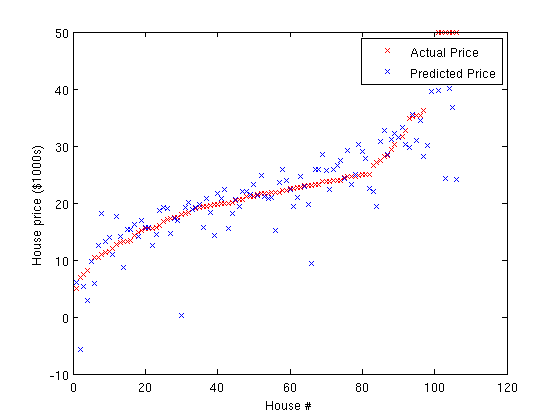
\includegraphics[scale=0.4]{figures/sample_figure.png}
     \caption{Inductance of oscillation winding on amorphous
      magnetic core versus DC bias magnetic field}
\label{fig-sample}
  \end{figure}
  The paper is organized as follows.
  The following section reviews the literature regarding robot localization with WiFi signal.
  In Sec.~\ref{sec-PF}, we formalize the problem.
  Section~\ref{sec-SD} thoroughly explains the proposed system.
  The experimentation and the results are  in Sec.~\ref{sec-EX}.
  We outline our observation and conclusions in the final section.

% \begin{itemize}
%   \item \sout{ubiquitous wifi information}
%   \item \sout{multipath effect}
%   \item \sout{no other infrasracture needed, low cost}
%   \item the acquired information is not reliable (maybe a figure can go here showing RSSI deviation in time)
%   \item conclusion: still an open problem due to the poor accuracy
% \end{itemize}
%
%
%
\section{\label{sec-RW}RELATED WORK}
  Indoor localization is an important problem in which an object of interest, i.e.\ a robot in our framework, suited with different sensors localizes itself in an indoor environment where there is no global positioning information is available.
  \textit{The importance of indoor localization where there is no reliable global positioning system is available.
  Maybe co-robots can be mentioned.}
  The indoor localization systems based WiFi signal can be categorized under two categories: fingerprinting and model-based~\cite{hossain2015survey}.
  We'll only cover the fingerprinting technique due to the increasing popularity of the technique.

  \subsection{Indoor Localization Based on Fingerprinting}
    A brief description for fingerprinting which had been surveyed many times~\cite{he2016wi, liu2007survey} with different scopes.
    Many of the previous systems employ spatial pattern of the fingerpr    Zee~\cite{rai2012zee}: off-the-shelf hw, crowdsourcing
    \lorem{}ints while others temporal pattern of the fingerprints.
    % UnLoc~\cite{wang2012no}: zero supervising, no training; heavily depends on landmark extraction and dead reckoning. (mobile device)
    % One of the recent advances is that to incorporate the hard-constraints induced by the environment infrasracture.
    UnLoc~\cite{wang2012no} is an examplary instance falling the former category.
    The system aims for incorporating hard-constraints of the environment (elevators, stairs, entrances) and the change in the fingerprint patterns; for instance, a dead zone for a specific AP\@.

    %% NO FP, mission abort!
    % EZ~\cite{chintalapudi2010indoor}: Microsoft, model-based, GA, Receiver gain differences, need at least $n$ number of APs.

    Particle filter~\cite{biswas2010wifi}: PF, dead reckoning
    \lorem{}
    % LiFS~\cite{yang2012locating}: no radio map required heavily depends on multiresolution mapping.
    While the previous work presented the belief of the robot pose with a set of particles, LiFS~\cite{yang2012locating} approximated the environment by a grid-based method.
    The grids are then transformed to \textit{stress-free floor plan} where the grids were clustered based on walking-distance among each other rather than physical distance; due to the fact that in indoor settings not every neighboring grids are accessible from one to another within one step.
    The fingerprints are then collected during a walk in the localization environment, as the proposed data acquisition algorithm labels fingerprints with the number of steps taken.
    The signal map were then constructed with the observed fingerprints with a Multidimensional scaling technique~\cite{borg2005modern}.
    % The fingerprints are then clustered with the same multiscaling algorithm, after a tedious preprosessing step.
    After acquiring fingerprint space and stress-free floor plan, the correspondence between two information was then calculated to map one to another; thus, spatial information was tied to fingerprints of the AP's.
    This work achieved comparable localization results but depending on

    Zee~\cite{rai2012zee}: off-the-shelf hw, crowdsourcing
    \lorem{}

    ArrayTrack~\cite{xiong2013arraytrack}: One of the best
    \lorem{}

    Walkie-Markie~\cite{shen2013walkie}: spatial-pattern
    \lorem{}

    SpotFi~\cite{kotaru2015spotfi}: One of the best
    \lorem{}

    %
    % FP~\cite{he2016wi}: FP Survey
    %
    % Calibration-free~\cite{hossain2015survey}: Calibration-free survey
    %
    % General wireless~\cite{liu2007survey}: High number of citations

  \subsection{Indoor Localization with Machine Learning}
    kNN:~\cite{liu2007survey}
    \lorem{}


    Neural networks:~\cite{dayekh2010cooperative}
    \lorem{}

    SVM:~\cite{wu2007location}
    \lorem{}

    Deep-Fi~\cite{wang2016csi}: Deep learning
    \lorem{}

    % \begin{itemize}
    %   \item{RSS Based}
    %   \item{CSI Based}
    %   \item{TDOA Based}
    %   \item{RTT Based}
    % \end{itemize}

    In the scope of WiFi localization systems, it is still an open problem in the field of robotics to deal with this problem with off-the-shelf AP's, while resulting relatively higher localization results than other applications where NLoS observation can happen anytime.

% \begin{itemize}
%   \item CSI-related special \\
%     hardware requirement
%   \item Propagation-modelling \\
%     multi-path effect difficult to model
%   \item Fingerprinting \\
%     An emerging area learning fingerprints is deep learning~\cite{gao2015channel}
% \end{itemize}



\section{\label{sec-PF}PROBLEM FORMULATION}
  \lorem{}
\section{\label{sec-SD}SYSTEM DESCRIPTION}
  \subsection{Offline Stage}

    \subsubsection{Data Acquisition}

    \subsubsection{Training}

  \subsection{Online Stage}

    \subsubsection{Inference}

    \subsubsection{Information Fusion}
    \lorem{}

\section{\label{sec-EX}EXPERIMENTATION}
  \subsection{Experimental Setup}
    \subsubsection{Hardware}
      % Fetch
    \subsubsection{Software}
      % ROS and Caffee
  \subsection{Results}
  \lorem{} 
  \lorem{}

\section{\label{sec-CO}CONCLUSIONS}
  \lorem{}

\addtolength{\textheight}{-12cm}   % This command serves to balance the column lengths
                                  % on the last page of the document manually. It shortens
                                  % the textheight of the last page by a suitable amount.
                                  % This command does not take effect until the next page
                                  % so it should come on the page before the last. Make
                                  % sure that you do not shorten the textheight too much.


\section*{ACKNOWLEDGMENT}
Turkish Government and stuff

\bibliographystyle{IEEEtran}
\bibliography{bibliography}

\end{document}
